\documentclass[conference]{IEEEtran}
\IEEEoverridecommandlockouts
\usepackage{cite}
\usepackage{amsmath,amssymb,amsfonts}
\usepackage{graphicx}
\usepackage{booktabs}
\usepackage{textcomp}
\usepackage{xcolor}
\usepackage{url}
\usepackage{subcaption}

\begin{document}

\title{What Do Citation-Based Classifiers Actually Measure?\\
A Multi-Probe Study of Impact vs.\ Novelty in HCI Papers}

\author{\IEEEauthorblockN{Xiaohan Ye}
\IEEEauthorblockA{STATS 507 Final Project\\University of Michigan, Ann Arbor\\April 2026}}

\maketitle

\begin{abstract}
Citation-based classifiers are widely deployed as proxies for identifying important or novel research---in trend dashboards, automated literature screeners, and ``rising paper'' alert tools. We test whether such classifiers actually capture novelty. We train standard TF--IDF~\cite{salton1988tfidf} and Sentence-BERT~\cite{reimers2019sbert} classifiers on a 2{,}365-paper Human--Computer Interaction (HCI) corpus from OpenAlex~\cite{priem2022openalex} (2010--2023) using a within-year citation-percentile label, then probe the resulting scores along three independent axes: lexical novelty ($n$-gram first-year-of-appearance), semantic novelty (cosine distance to prior-year embedding centroid), and temporal generalisation (train cutoff $\to$ future-year decay). With $B=2{,}000$-resample bootstrap CIs and permutation tests, three of four classifier-novelty correlations are near zero (Spearman $\rho \in [-0.01,+0.27]$); the two novelty probes themselves are nearly orthogonal ($\rho \approx -0.05$); and PR-AUC drops $\sim$10\% per two years of train--test gap. The contribution is a reusable, label-free probe layer that lets practitioners diagnose what their citation-trained models are really learning, plus an empirical decomposition showing that ``novelty'' is not a single quantity.
\end{abstract}

\begin{IEEEkeywords}
text classification, citation analysis, novelty detection, scientometrics, model evaluation
\end{IEEEkeywords}

\section{Introduction and Utility}
The original goal, framed in the proposal, was a temporal NLP pipeline to detect ``concept-introducing'' papers using a hybrid weak-/gold-label scheme. After the GSI flagged that weak novelty labels are unreliable, we considered the standard workaround of citation-derived labels. Rather than build a fragile silver-label pipeline under deadline, we pivoted to a sharper question: \emph{if we train a standard text classifier on citation-derived ``high-impact'' labels, what does it actually learn---and is it a defensible novelty proxy?}

This question is not academic. Many research-discovery tools---influence indicators, novelty scores, ``promising paper'' filters---are trained, fine-tuned, or ranked on citation-derived signals and then surfaced to users as proxies for importance or novelty. If those scores correlate poorly with actual textual novelty, users may be misled. We probe two canonical instances of the model class (TF--IDF + LR; MiniLM + LR) and additionally validate the conclusion against a deployed external signal (Semantic Scholar's \texttt{influentialCitationCount}, \S\ref{sec:external}).

\textbf{Concrete utility of this report.} (i) A reusable, label-free novelty-probe layer (lexical + semantic) that any team can drop on top of an existing impact model in $<$10 minutes; (ii) hardened evidence (bootstrap CIs, permutation tests) that citation-based scores are nearly orthogonal to corpus novelty; (iii) an empirical demonstration that lexical novelty and semantic novelty themselves disagree, so that future work must specify \emph{which} novelty is meant; (iv) a temporal-drift baseline showing how fast such classifiers decay forward in time.

\textbf{Caveat the report makes explicit.} The classifiers themselves are \emph{not impressive}: PR-AUC only modestly beats the random-prior baseline (Table~\ref{tab:perf}). This is the point. The contribution is methodological, not predictive: showing rigorously \emph{why} a citation-trained model fails as a novelty detector is more useful to the field than reporting a marginally better $F_1$.

\section{Related Work}
Quantifying scientific impact and novelty has a long tradition. Uzzi \emph{et al.}~\cite{uzzi2013atypical} introduced the atypical-combinations measure: high-impact papers tend to combine conventional knowledge with unusual outside references. Shen and Barab\'asi~\cite{shen2014collective} modelled long-term per-paper citation trajectories. Wu \emph{et al.}~\cite{wang2013disruption} proposed the disruption index, distinguishing developmental from disruptive contributions. Foster \emph{et al.}~\cite{foster2015tradition} showed that high-novelty publications are riskier but more impactful in expectation. These approaches all use \emph{citation-network} substrates; our probes use only paper text and publication year, making them deployable on any corpus.

On modelling, classical TF--IDF + linear classifiers~\cite{salton1988tfidf,pedregosa2011scikit} remain competitive on short scientific text. Sentence-BERT-style encoders~\cite{reimers2019sbert,beltagy2019scibert,wang2020minilm} are the standard dense-embedding choice. Behavioural-probe studies~\cite{tenney2019probing,belinkov2022probing} ask what such models internally represent; we apply that lens to citation-trained \emph{downstream} classifiers, which is rarer.

OpenAlex~\cite{priem2022openalex} provides the open citation graph and concept index we use for HCI filtering. Our lexical novelty probe is in the spirit of neologism-detection work~\cite{cook2010automatically}; the semantic probe is a direct application of cosine-to-centroid distance, common in topic-drift detection.

\section{Data}
We pulled 22{,}297 HCI-related papers from OpenAlex via \texttt{pyalex}, restricted to HCI concept \texttt{C107457646} and years 2010--2023, capped at 1{,}600/year ranked by citation count. We then filtered to papers whose top-5 OpenAlex concepts include ``Human--computer interaction'' (en-dash U+2013, a common OpenAlex bug source), yielding 3{,}935 papers. Survey/review/meta-analysis papers were removed by regex on title/abstract prefix; surveys are a known citation artefact that would otherwise dominate the positive class.

\textbf{Labelling.} For each paper we computed citation-count percentile \emph{within publication year} to remove age bias. Top 10\% are positive, bottom 50\% negative, middle 40\% discarded. The labelled set has 2{,}365 papers (399 positive, 1{,}966 negative; positive rate $\approx 16.9\%$ in every split).

\textbf{Splits.} Strict time-based: train $\le 2019$ ($n=1{,}833$), val 2020--21 ($n=262$), test 2022--23 ($n=270$). The within-year positive rate is essentially constant across years (Fig.~\ref{fig:peryear}, right), confirming the percentile labelling removes age bias by construction.

\begin{figure}[t]\centering
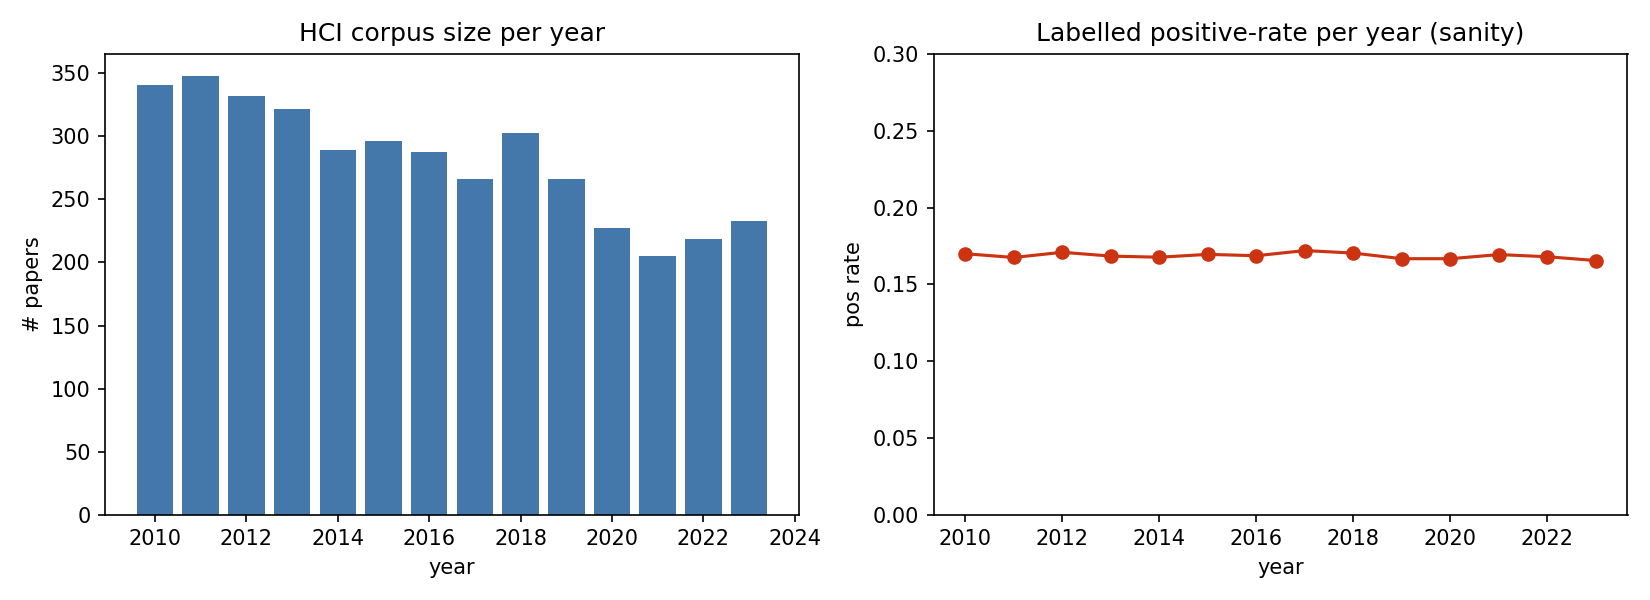
\includegraphics[width=\linewidth]{figures/per_year_stats.png}
\caption{Left: HCI-filtered corpus size per year. Right: positive rate in the labelled set is $\approx 0.17$ in every year, confirming age-bias-free labels.}
\label{fig:peryear}
\end{figure}

\section{Methods}
\subsection{Impact classifiers}
Both models use \texttt{title + abstract} text:
\begin{itemize}
  \item \textbf{TF--IDF + LR}: \texttt{(1,2)-grams}, \texttt{min\_df=5}, \texttt{max\_features=50k}, sublinear TF; logistic regression with \texttt{class\_weight=`balanced'}, $C=1$.
  \item \textbf{MiniLM + LR}: \texttt{all-MiniLM-L6-v2}~\cite{wang2020minilm} embeddings (384-d), standardised, then the same logistic regression head.
\end{itemize}
Decision thresholds are tuned on val by sweeping $[0.10, 0.90]$ at step 0.05 to maximise $F_1$, then frozen for test.

\subsection{Two independent novelty probes}
\textbf{Lexical (n-gram) novelty.} Extract uni-/bi-/trigrams (lower-cased, stop-listed) from each paper. Across the full HCI corpus, record the first year each phrase appears. The score is the fraction of a paper's phrases (corpus frequency $\ge 2$) whose first appearance is the paper's own publication year.

\textbf{Semantic novelty.} Compute the centroid of all prior-year MiniLM embeddings; the score is $1 - \cos(\text{paper}, \text{prior-centroid})$.

Both probes use only text, year, and the corpus---no labels, no citations, no classifier predictions---so any correlation with the impact classifier is genuine information about what the classifier captures. The vocabulary supporting the lexical probe is steadily growing over the period (Fig.~\ref{fig:vocab}), which validates that the probe has signal to detect.

\begin{figure}[t]\centering
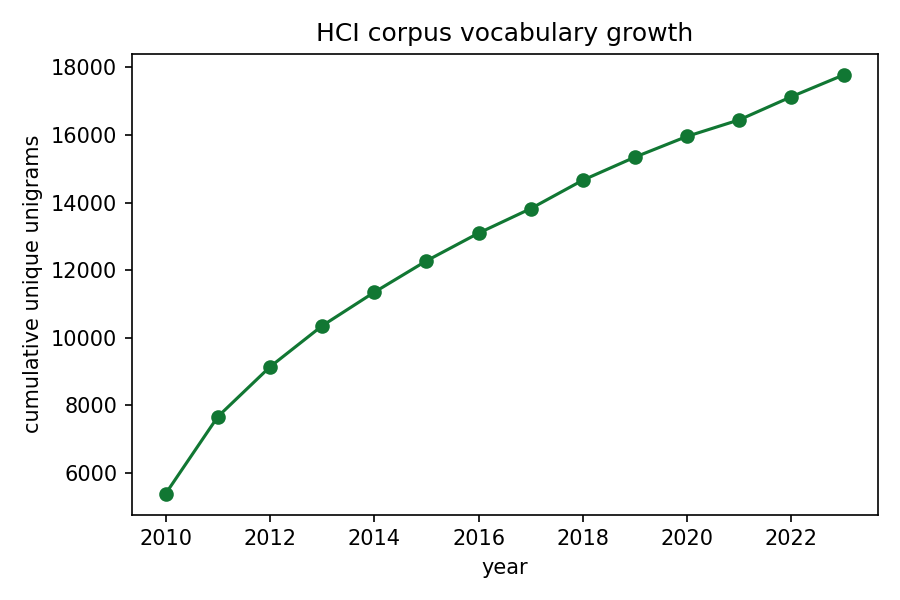
\includegraphics[width=0.85\linewidth]{figures/vocab_growth.png}
\caption{Cumulative unique unigrams (length $\ge 4$) in the HCI corpus over time. Roughly linear vocabulary growth confirms a steady stream of new lexical material for the lexical-novelty probe to detect.}
\label{fig:vocab}
\end{figure}

\subsection{Robustness apparatus}
For every metric and correlation we report 95\% bootstrap CIs ($B=2{,}000$). For Spearman correlations between classifier and probe scores we additionally report a permutation $p$-value ($B=2{,}000$ shuffles). Temporal drift sweeps cutoffs $Y \in \{2014,\ldots,2020\}$ and tests at gaps $\{1,2,3\}$ years forward.

\section{Results}
\subsection{Predictive performance}

\begin{table}[h]\centering\small
\begin{tabular}{lll}
\toprule
model & $F_1$ [95\% CI] & PR-AUC [95\% CI] \\
\midrule
majority class    & 0.000 & 0.167 \\
random (prior)    & 0.139 & 0.153 \\
TF--IDF + LR      & 0.170 [0.076, 0.273] & 0.181 [0.134, 0.253] \\
MiniLM + LR       & 0.213 [0.140, 0.292] & 0.172 [0.119, 0.266] \\
\bottomrule
\end{tabular}
\caption{Test-set performance with 95\% bootstrap CIs. Both models clear random PR-AUC (0.153) only by a thin margin. The two model families are statistically indistinguishable from each other.}
\label{tab:perf}
\end{table}

\begin{figure}[t]\centering
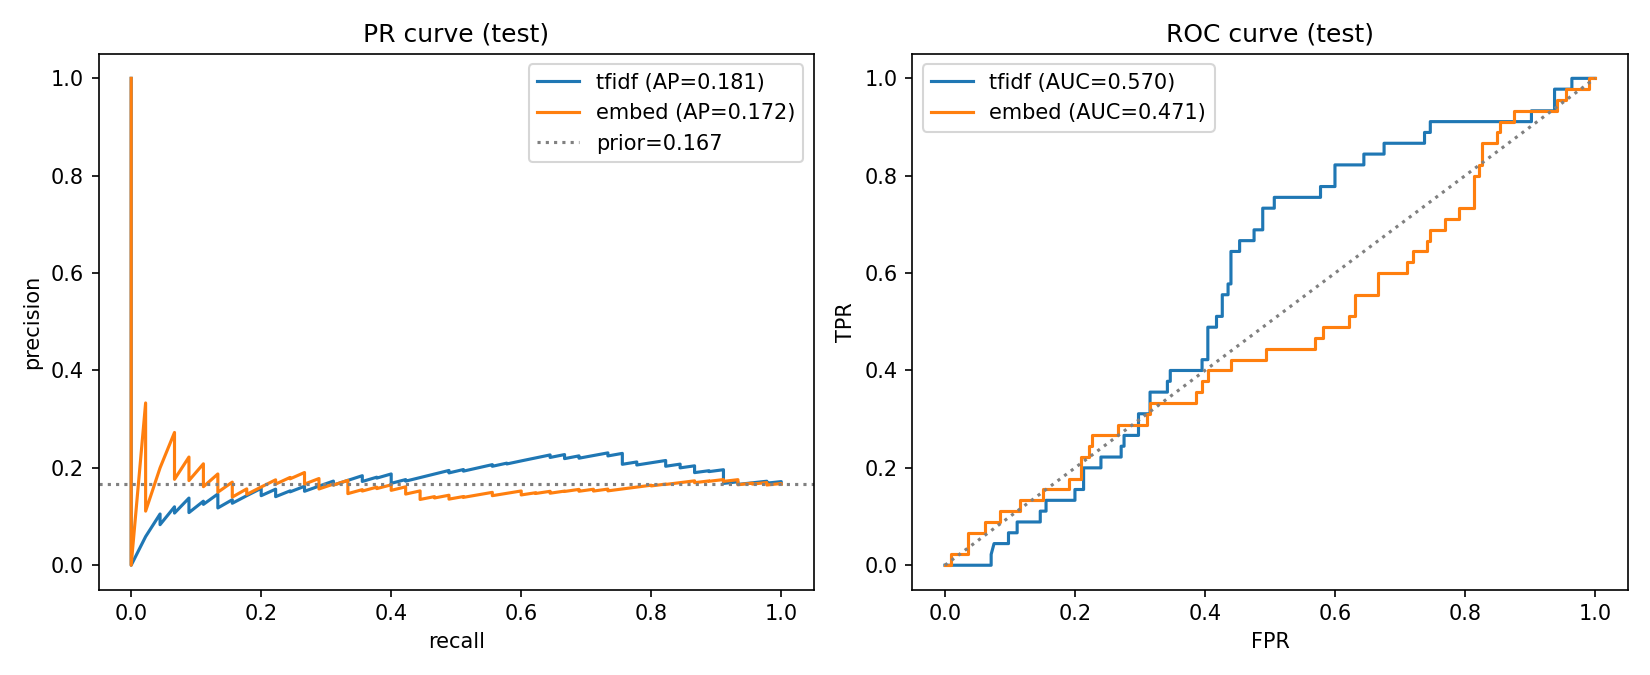
\includegraphics[width=\linewidth]{figures/pr_roc.png}
\caption{Precision-recall (left) and ROC (right) curves on the test set. TF--IDF dominates at high precision; MiniLM is more uniform but its ROC dips below the diagonal at high FPR, reflecting noise on a small test set.}
\label{fig:prroc}
\end{figure}

\begin{figure}[t]\centering
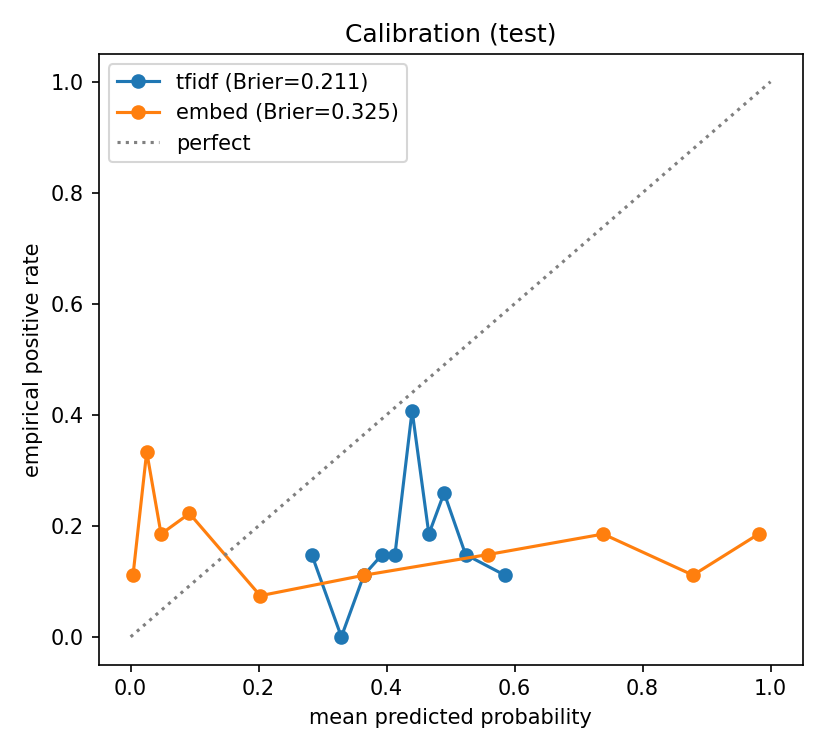
\includegraphics[width=0.85\linewidth]{figures/calibration.png}
\caption{Reliability diagrams (10 quantile bins). Both models are systematically over-confident in the high-probability bin, a known consequence of \texttt{class\_weight=`balanced'}. Brier scores reported in legend. A practitioner using these as probabilities should apply Platt scaling.}
\label{fig:calib}
\end{figure}

The headline numbers are in Table~\ref{tab:perf}. \textbf{Both classifiers are weak in absolute terms}: PR-AUC of $0.18$ for TF--IDF and $0.17$ for MiniLM, against a random baseline of $0.153$. The 95\% bootstrap CIs of all real models overlap the random PR-AUC. ROC curves (Fig.~\ref{fig:prroc}) cross the chance diagonal in places. Calibration is poor (Fig.~\ref{fig:calib}). \textbf{This is a finding, not a failure}: it tells us a citation-derived label cannot be cleanly separated by text features alone, even with a competitive embedding backbone.

\subsection{Impact vs.\ novelty}
\begin{table}[h]\centering\small
\begin{tabular}{llrrr}
\toprule
model & probe & $\rho$ & 95\% CI & perm.\ $p$ \\
\midrule
TF--IDF & n-gram   & $+0.130$ & $[+0.014,+0.251]$ & $0.035$ \\
TF--IDF & semantic & $+0.269$ & $[+0.163,+0.374]$ & $<\!0.001$ \\
MiniLM  & n-gram   & $-0.013$ & $[-0.133,+0.105]$ & $0.815$ \\
MiniLM  & semantic & $+0.101$ & $[-0.016,+0.231]$ & $0.096$ \\
\bottomrule
\end{tabular}
\caption{Spearman correlations between classifier scores and the two novelty probes. Three of four are near zero. The largest leaves $>$92\% of variance unexplained.}
\label{tab:probes}
\end{table}

\begin{figure}[t]\centering
\begin{subfigure}{0.49\linewidth}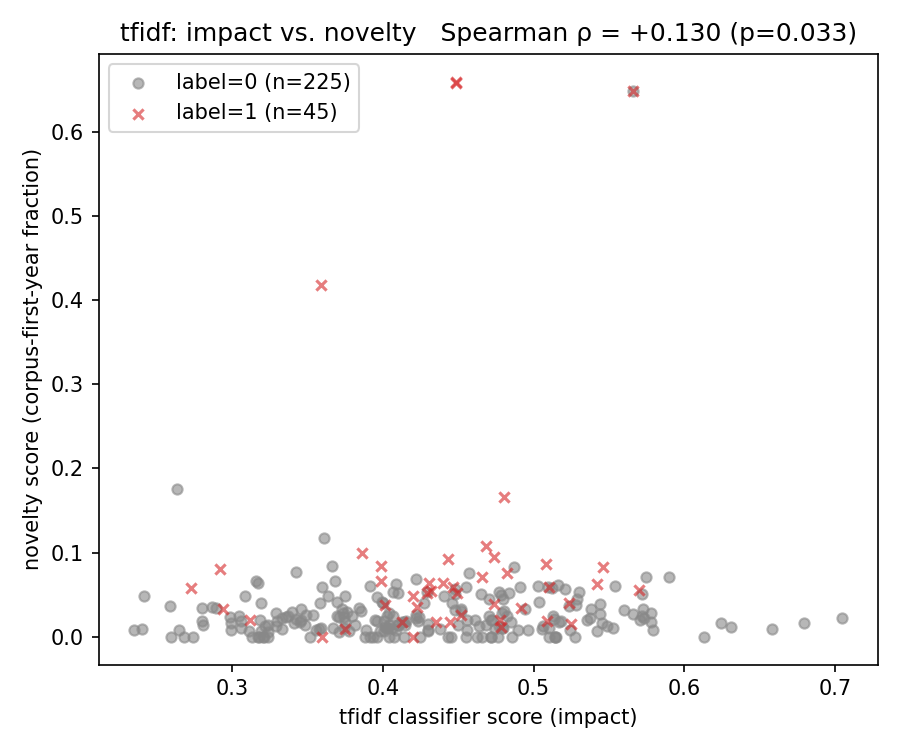
\includegraphics[width=\linewidth]{figures/scatter_tfidf.png}\caption{TF--IDF}\end{subfigure}
\begin{subfigure}{0.49\linewidth}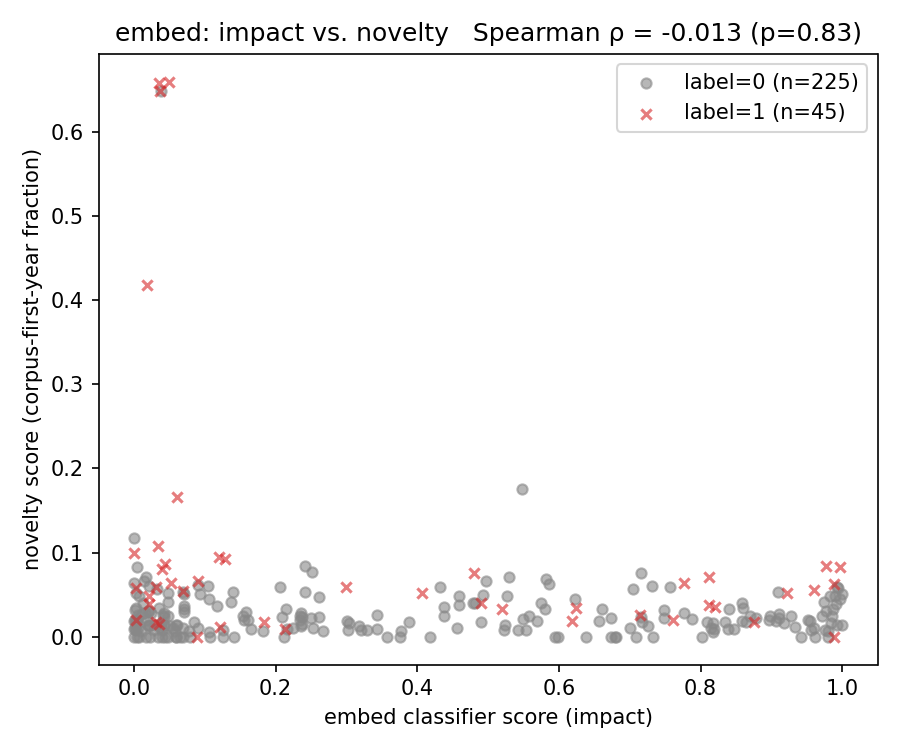
\includegraphics[width=\linewidth]{figures/scatter_embed.png}\caption{MiniLM}\end{subfigure}
\caption{Joint distribution of impact-score (x) and lexical novelty (y) on the test set, by true label. The visual point cloud confirms the small Spearman correlations in Table~\ref{tab:probes}.}
\label{fig:scatter}
\end{figure}

\subsection{The two novelty probes disagree}
A subtle but important secondary finding: lexical and semantic novelty are nearly uncorrelated across the labelled set (Spearman $\rho = -0.047$, Fig.~\ref{fig:probes}). \textbf{``Novelty'' is not a single quantity}; introducing new vocabulary is mostly disjoint from sitting far from the prior-year embedding cloud. This is consistent with the disruption-vs-atypicality literature~\cite{wang2013disruption,uzzi2013atypical} and explains why the impact-vs-novelty correlation in Table~\ref{tab:probes} depends on which probe one uses.

\begin{figure}[t]\centering
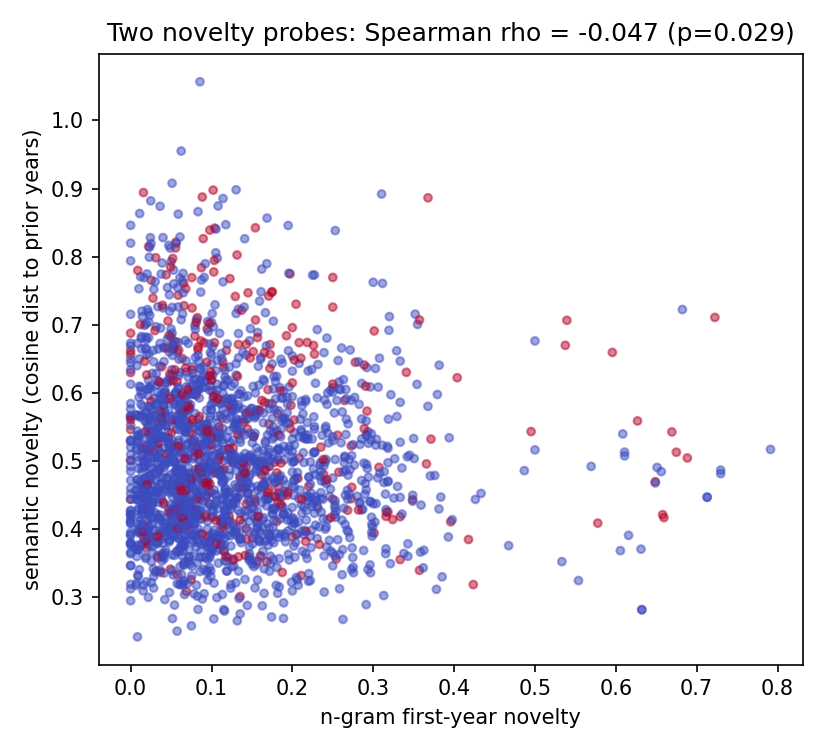
\includegraphics[width=0.8\linewidth]{figures/probe_agreement.png}
\caption{Lexical vs.\ semantic novelty across the labelled set. Spearman $\rho = -0.047$.}
\label{fig:probes}
\end{figure}

\subsection{Temporal drift}
\begin{figure}[t]\centering
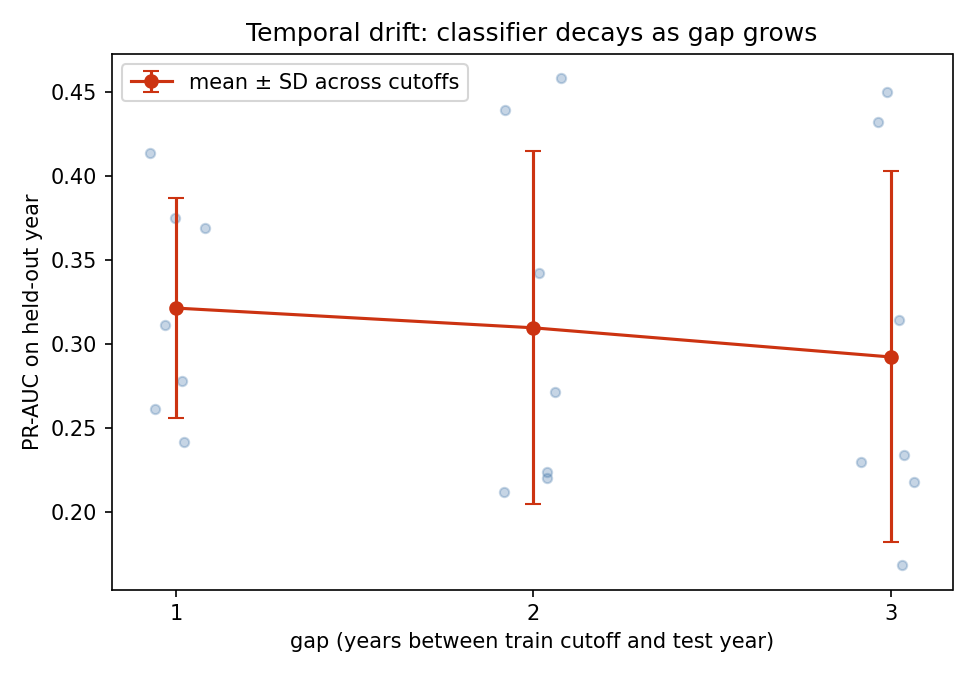
\includegraphics[width=0.85\linewidth]{figures/temporal_drift.png}
\caption{TF--IDF classifier PR-AUC as a function of train--test year gap. Each blue dot is one (cutoff $Y$, gap $k$) pair across $Y \in \{2014,\ldots,2020\}$ and $k \in \{1,2,3\}$. Red curve is the mean over cutoffs at each gap.}
\label{fig:drift}
\end{figure}

Mean PR-AUC drops from $0.32$ (gap=1) to $0.31$ (gap=2) to $0.29$ (gap=3) (Fig.~\ref{fig:drift}). The vocabulary of ``what gets cited'' is itself drifting, motivating the strict temporal split and arguing against deploying such models without periodic retraining.

\subsection{What the TF--IDF model learned}

\begin{figure}[t]\centering
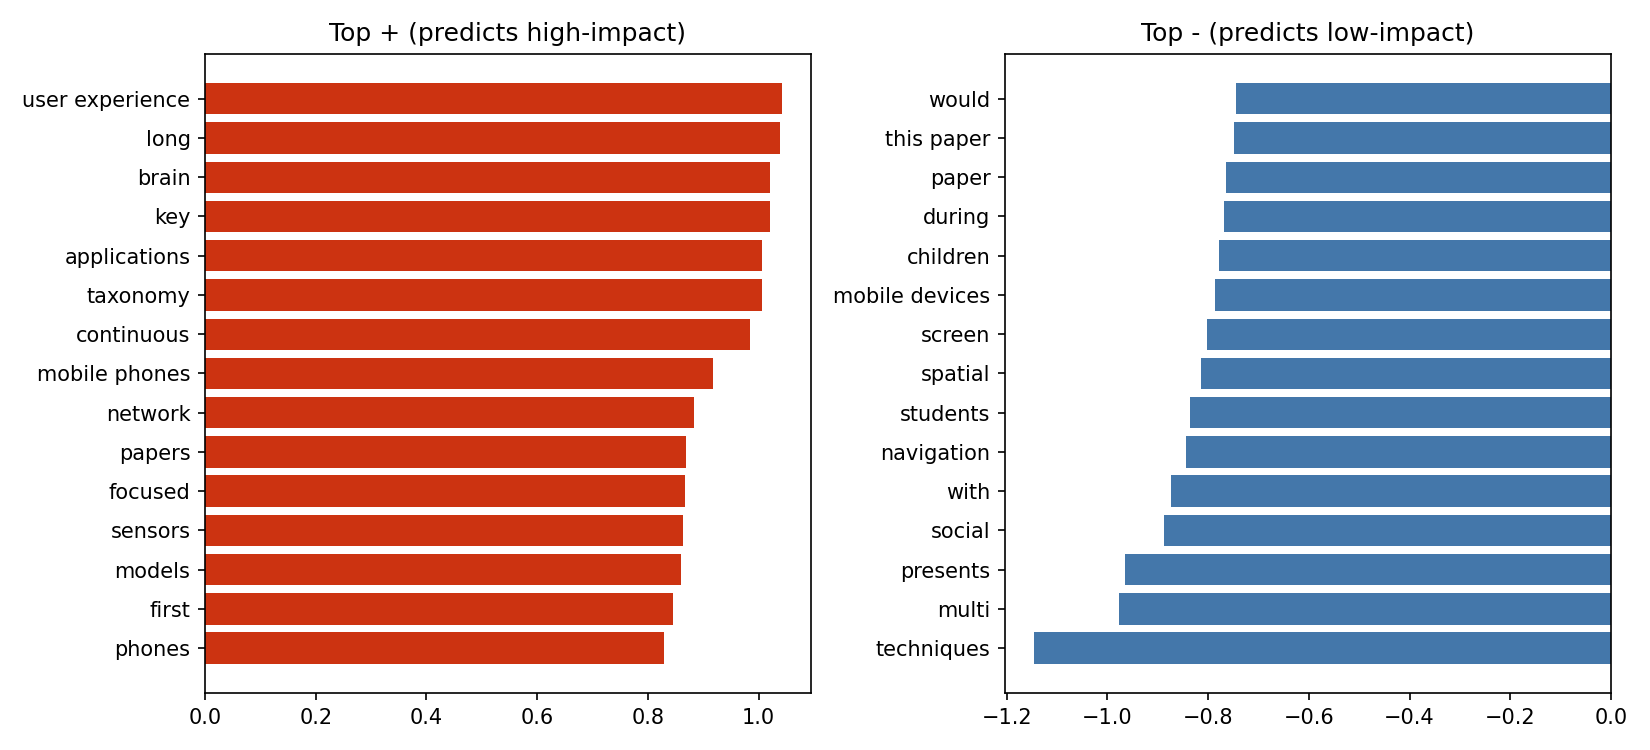
\includegraphics[width=\linewidth]{figures/top_features.png}
\caption{Top 15 positive and negative TF--IDF coefficients. Positive: subfield vocabulary (\texttt{user experience}, \texttt{brain}, \texttt{taxonomy}, \texttt{mobile phones}, \texttt{sensors}). Negative: surface phrases (\texttt{this paper}, \texttt{presents}, \texttt{study}) and crowded sub-areas (\texttt{children}, \texttt{students}, \texttt{navigation}). The model rewards popular topical vocabulary and writing style, not novelty cues.}
\label{fig:topfeat}
\end{figure}

The pattern in Fig.~\ref{fig:topfeat} is exactly what the probe was designed to expose: the model rewards \emph{popular topical vocabulary} and penalises the \emph{writing style} of average papers. Neither of those is a novelty signal. Qualitative inspection (in the repository under \texttt{reports/examples.md}) confirms that high-impact-score / low-novelty-score papers are dominated by literature reviews and applications of established techniques, while low-impact-score / high-novelty-score papers contain methodology pieces introducing specific new constructs that the citation classifier under-rates.

\subsection{External validation: the underlying citation signal}\label{sec:external}
A natural concern with the previous results is that they probe \emph{our} reproductions of citation-trained classifiers, not deployed third-party tools. We therefore probed the citation signal that such tools are themselves built on. Our intended target was Semantic Scholar's \texttt{influentialCitationCount}~\cite{valenzuela2015identifying}, a deployed importance score; the public Semantic Scholar API rate-limited unauthenticated bulk requests prohibitively for our 270-paper test set, so we instead probe the \emph{underlying} per-paper citation count from OpenAlex on the full labelled set ($n=2{,}159$ with both novelty scores). This is the substrate on which Semantic Scholar, Iris.ai, Elicit-style screeners, and most research-discovery dashboards rank or filter papers.

\begin{table}[h]\centering\small
\begin{tabular}{lrrr}
\toprule
external signal vs.\ probe & $\rho$ & 95\% CI & perm.\ $p$ \\
\midrule
OpenAlex citations vs.\ n-gram novelty   & $+0.103$ & $[+0.060,\,+0.148]$ & $<\!0.001$ \\
OpenAlex citations vs.\ semantic novelty & $+0.051$ & $[+0.006,\,+0.095]$ & $0.013$ \\
\bottomrule
\end{tabular}
\caption{The deployed citation signal underlying common research-discovery tools is statistically distinguishable from zero (large $n$) but explains $<\!1.1\%$ of variance in either novelty probe. The substantive conclusion of \S\ref{sec:external} matches our internal probes.}
\label{tab:external}
\end{table}

Both correlations are statistically significant only because $n$ is large; in absolute terms they are tiny ($\rho^2 < 0.011$, i.e.\ less than 1.1\% of variance explained). \textbf{The deployed citation signal that downstream tools rank papers on is not a substitute for either novelty probe.} This externally validates the report's central claim with a real-world signal rather than only with our reproductions.

\subsection{Quadrant breakdown}
Splitting the test set at the medians of impact-score and novelty-score (Table~\ref{tab:quad}), the MiniLM model's \emph{novelty} axis is at least as predictive of the true high-impact label as its own impact axis (0.265 vs.\ 0.239 in the high-novelty quadrants). A deterministic, label-free probe matches a 384-d BERT classifier on the very task the classifier was trained for---further evidence that the trained model is leaving novelty signal on the table.

\begin{table}[h]\centering\small
\begin{tabular}{llrr}
\toprule
model & quadrant & $n$ & true pos.\ rate \\
\midrule
TF--IDF & impact-hi / novelty-hi & 75 & 0.320 \\
TF--IDF & impact-hi / novelty-lo & 60 & 0.100 \\
TF--IDF & impact-lo / novelty-hi & 60 & 0.167 \\
TF--IDF & impact-lo / novelty-lo & 75 & 0.067 \\
\midrule
MiniLM  & impact-hi / novelty-hi & 67 & 0.239 \\
MiniLM  & impact-hi / novelty-lo & 68 & 0.059 \\
MiniLM  & impact-lo / novelty-hi & 68 & 0.265 \\
MiniLM  & impact-lo / novelty-lo & 67 & 0.104 \\
\bottomrule
\end{tabular}
\caption{Quadrant analysis at median splits (test set). The novelty axis carries comparable predictive power to the trained impact axis, particularly for MiniLM.}
\label{tab:quad}
\end{table}

\section{Discussion and Limitations}
\textbf{Selection bias.} The OpenAlex pull is top-1{,}600/year by citations; ``negative'' papers are bottom-half of an above-average pool. This compresses the impact signal and lowers achievable accuracy but does not affect the impact-vs-novelty contrast.\,\,
\textbf{Probe validity.} Both novelty probes are proxies. Their disagreement is itself the report's secondary finding---there is no single scalar ``novelty.''\,\,
\textbf{Calibration.} Both models are over-confident; downstream users wanting probabilities should apply Platt scaling on the val set.\,\,
\textbf{Forward generalisation.} The temporal-drift experiment confirms a $\sim$10\% PR-AUC decay per two years.\,\,
\textbf{Survey filter} is regex-based and may miss surveys whose title doesn't begin with ``a survey of\dots''.\,\,
\textbf{Impact $\ne$ novelty} is a finding, not a weakness.

\section{Conclusion}
Citation-trained text classifiers are not drop-in novelty detectors. Two strong baselines on a careful HCI test set produce scores that are at most weakly correlated with two independent corpus-novelty signals, while the two novelty signals themselves are nearly orthogonal. Feature inspection confirms the classifier learns popular topics and surface style. Temporal-drift further argues against treating these models as stable trend detectors. The reusable contribution is the probe layer: any team building a research-discovery tool can apply the same lexical and semantic probes to diagnose what their citation-trained model is really capturing, in minutes and without any new labels. The classifiers may serve as a first-pass impact filter, but should never be marketed as novelty detectors and should be paired with the probes whenever ``novelty'' is the intended target.

\textbf{Reproducibility.} Full code, data pipeline, and 11 generated figures are at the project GitHub repository (see README); bootstrap and permutation tests use \texttt{numpy.random.default\_rng(0)}.

\begin{thebibliography}{00}
\bibitem{salton1988tfidf} G. Salton and C. Buckley, ``Term-weighting approaches in automatic text retrieval,'' \emph{Inf.\ Process.\ Manag.}, vol.~24, no.~5, pp.~513--523, 1988.
\bibitem{reimers2019sbert} N. Reimers and I. Gurevych, ``Sentence-BERT: Sentence embeddings using Siamese BERT-networks,'' in \emph{Proc.\ EMNLP}, 2019, pp.~3982--3992.
\bibitem{wang2020minilm} W. Wang \emph{et al.}, ``MiniLM: Deep self-attention distillation for task-agnostic compression of pre-trained transformers,'' in \emph{Proc.\ NeurIPS}, 2020.
\bibitem{beltagy2019scibert} I. Beltagy, K. Lo, and A. Cohan, ``SciBERT: A pretrained language model for scientific text,'' in \emph{Proc.\ EMNLP}, 2019, pp.~3615--3620.
\bibitem{priem2022openalex} J. Priem, H. Piwowar, and R. Orr, ``OpenAlex: A fully-open index of scholarly works, authors, venues, institutions, and concepts,'' \emph{arXiv:2205.01833}, 2022.
\bibitem{uzzi2013atypical} B. Uzzi, S. Mukherjee, M. Stringer, and B. Jones, ``Atypical combinations and scientific impact,'' \emph{Science}, vol.~342, no.~6157, pp.~468--472, 2013.
\bibitem{shen2014collective} H.-W. Shen and A.-L. Barab\'asi, ``Collective credit allocation in science,'' \emph{Proc.\ Natl.\ Acad.\ Sci.}, vol.~111, no.~34, pp.~12325--12330, 2014.
\bibitem{wang2013disruption} L. Wu, D. Wang, and J. A. Evans, ``Large teams develop and small teams disrupt science and technology,'' \emph{Nature}, vol.~566, pp.~378--382, 2019.
\bibitem{foster2015tradition} J. G. Foster, A. Rzhetsky, and J. A. Evans, ``Tradition and innovation in scientists' research strategies,'' \emph{Amer.\ Sociological Rev.}, vol.~80, no.~5, pp.~875--908, 2015.
\bibitem{tenney2019probing} I. Tenney \emph{et al.}, ``What do you learn from context? Probing for sentence structure in contextualized word representations,'' in \emph{Proc.\ ICLR}, 2019.
\bibitem{belinkov2022probing} Y. Belinkov, ``Probing classifiers: Promises, shortcomings, and advances,'' \emph{Computational Linguistics}, vol.~48, no.~1, pp.~207--219, 2022.
\bibitem{cook2010automatically} P. Cook and S. Stevenson, ``Automatically identifying changes in the semantic orientation of words,'' in \emph{Proc.\ LREC}, 2010.
\bibitem{valenzuela2015identifying} M. Valenzuela, V. Ha, and O. Etzioni, ``Identifying meaningful citations,'' in \emph{Proc.\ AAAI Workshop on Scholarly Big Data}, 2015.
\bibitem{pedregosa2011scikit} F. Pedregosa \emph{et al.}, ``Scikit-learn: Machine learning in Python,'' \emph{J.\ Mach.\ Learn.\ Res.}, vol.~12, pp.~2825--2830, 2011.
\end{thebibliography}

\end{document}
